\documentclass[12pt, a4paper]{ctexart}

\usepackage{geometry}
\geometry{margin=2.5cm}
\usepackage{amsmath, amssymb}
\usepackage{graphicx}
\usepackage{booktabs}
\usepackage{caption}
\usepackage{subcaption}
\usepackage{float}
\usepackage{algorithm}
\usepackage{algpseudocode}
\usepackage[hidelinks]{hyperref}
\usepackage{xcolor}

\graphicspath{{../results/figures/}}
\captionsetup{font=small}

\title{基于尺度自标定的米粒计数方法：\\自适应标记控制分水岭与形状先验校正}
\author{数字图像处理课程作业}
\date{\today}

\begin{document}
\maketitle

\begin{abstract}
米粒计数的核心困难不在于分割前景，而在于分离相互粘连的米粒。本文提出 ASW-SPC
(Adaptive-Scale Watershed with Shape-Prior Correction)：先从图像自身估计单粒米的面积与形状先验，
再以该尺度驱动标记控制分水岭的种子生成，最后用米粒的凹性先验对分割结果做校正。
方法的全部尺度参数均由图像自标定得到，不含手工设定的像素常数。
在三个数据集（51 张真实照片、40 张粘连度可控的合成图、719 张低分辨率图像）上，
本方法的平均绝对误差分别为 5.92、1.77、3.32 粒。
在粘连场景下相对朴素连通域计数误差降低约 13 倍，且在三个数据集上均未出现灾难性失败。
本文同时给出与零样本 SAM 3 的对比：SAM 3 在提示词选对时精度更高，
但五个同样合理的提示词中有三个会在合成粘连集上静默失效，而挑选提示词本身需要标注数据。
本文亦如实报告所提方法在无粘连场景下并不优于简单基线这一局限。
\end{abstract}

\section{引言}

给定一张散落米粒的图像，自动数出米粒数目是一个典型的“分割—计数”任务。
在米粒互不接触时，该问题用经典流水线即可解决：灰度化、Otsu 阈值分割、连通域标记，
连通域数目就是米粒数。真正的困难出现在米粒相互接触时——多粒米会融合成一个连通域，
计数随之系统性偏低。

这一困难并非本文虚构。Kurade 等人在 \emph{Foods} 2023 上发表的米质评价系统\cite{kurade2023}
采用了教科书式的“形态学腐蚀取标记 + 分水岭”方案，却在论文中明确写道：
分水岭算法无法分离相互接触的米粒，因此这些米粒被从数据集中剔除；
其成像方案也刻意将 80 粒米均匀摊开、使其互不接触。
换言之，一篇已发表的工作选择了回避而非解决这一问题。本文正面处理它。

\subsection{主要工作}

\begin{enumerate}
  \item \textbf{尺度自标定}：以连通域面积在对数域的核密度主峰估计单粒米面积 $A_0$，
        并据此导出短轴、凸实度（solidity）、长宽比等形状先验。所有后续判据都以这些量为单位，
        因此方法不含随分辨率失效的像素常数。
  \item \textbf{数据驱动的二值化选择}：不预设颜色通道、阈值类别数与前景极性，
        而是构造候选集合并用“单粒一致性 $\times$ 局部对比度”打分自动选择。
  \item \textbf{基于凹性的粘连判定与异物剔除}：多粒米粘连必然在接触处留下凹颈，
        因此“比单粒更凸的大区域”不可能是米粒团。该判据同时解决了参照硬币被误计为数十粒米的问题。
  \item \textbf{可测量性门限}：当标定出的米粒宽度小到凸实度不再可测时，分割阶段主动弃权。
        这一条来自实测：米粒短轴小于约 $4.5$ 像素时，凸实度的离散化噪声几乎翻倍。
  \item \textbf{可控粘连度的合成基准}：用单粒米图像合成粘连度从 0\% 到 80\% 的场景，
        真值由构造过程精确给出，使“误差随粘连度的变化”可被直接测量。
\end{enumerate}

\section{相关工作}

\textbf{阈值与连通域。} Otsu 方法\cite{otsu1979}通过最大化类间方差自动选取全局阈值，
是灰度分割的标准手段。配合连通域标记即可完成非粘连场景的计数，但对粘连无能为力。

\textbf{分水岭及其过分割问题。} 分水岭变换\cite{vincent1991}将灰度图视为地形并模拟淹没过程，
天然适合分离粘连目标，但直接使用会因局部极值过多而严重过分割。
标记控制分水岭通过预先指定种子缓解该问题，
而种子如何生成正是各方法的分野：常见做法是对距离变换取固定比例阈值，或对二值图做形态学腐蚀\cite{kurade2023}。
本文将说明这两种固定尺度的做法为何在实际图像上失效。

\textbf{凹点与椭圆拟合。} 另一类思路直接在轮廓上寻找粘连处的凹点并配对切分，
或用椭圆近似粘连米粒的轮廓\cite{compag2019, wheat2025}，几何上可解释，
但依赖轮廓质量，对低分辨率图像不稳健。

\textbf{深度学习。} 以 SAM 3\cite{sam3} 为代表的开放词表分割模型可由文本提示直接给出实例掩膜，
无需针对任务训练。本文第 \ref{sec:sam3} 节将其作为对照，并讨论其代价。

\section{方法}

图 \ref{fig:pipeline} 给出总体流程。记二值前景为 $M$，其连通域集合为 $\{R_i\}$，
面积为 $S_i$，凸实度为 $\rho_i$，长短轴为 $a_i, b_i$。

\begin{figure}[H]
  \centering
  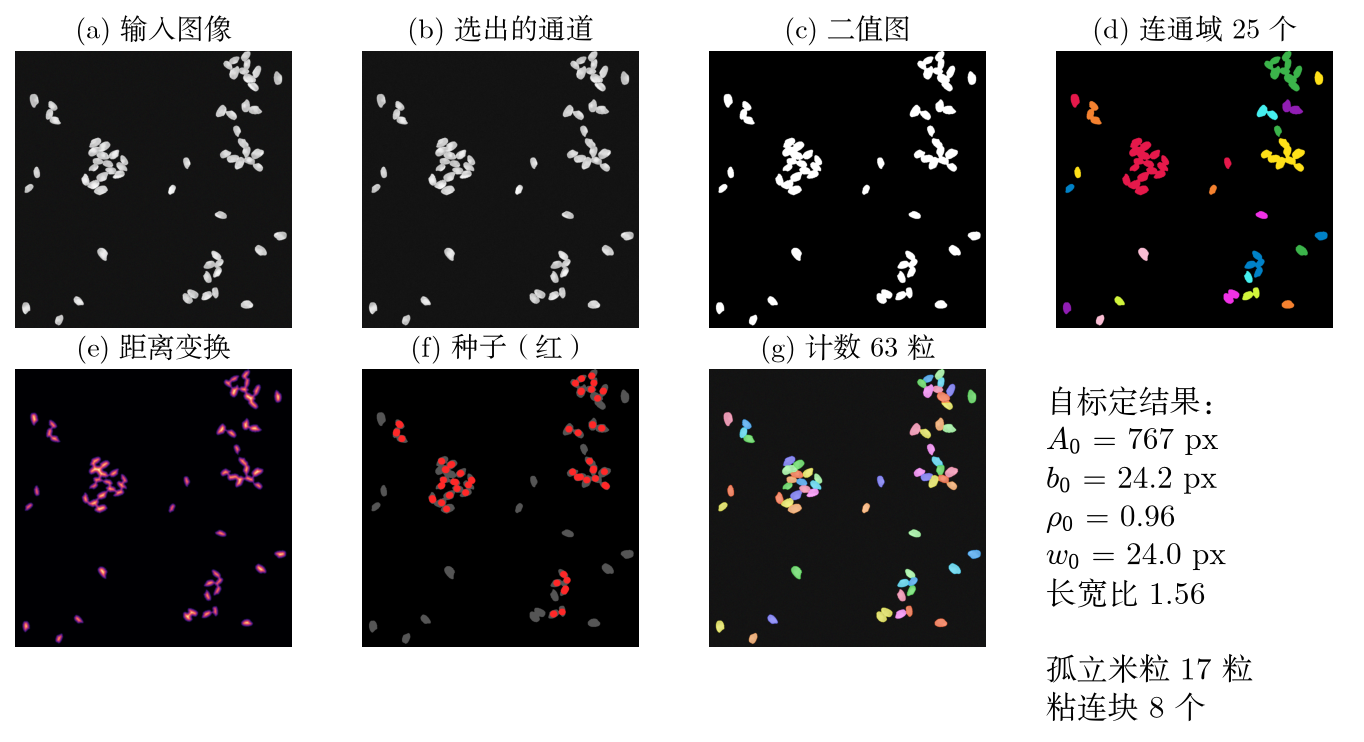
\includegraphics[width=\textwidth]{pipeline_synthetic.png}
  \caption{ASW-SPC 总体流程。(a) 输入；(b) 自动选出的通道与阈值方案；(c) 清理后的二值掩膜；
  (d) 连通域标记；(e) 距离变换；(f) 仅在粘连块内生成的自适应种子（红）；(g) 最终计数结果。
  右下列出全部由图像自标定得到的尺度与形状先验。}
  \label{fig:pipeline}
\end{figure}

\subsection{候选二值化与数据驱动选择}

真实场景常含三个以上灰度层次（桌面、衬布、米粒），两类 Otsu 的假设未必成立；
前景是“亮”还是“暗”也随衬布颜色而变。因此本文不固定这些选择，而是构造候选集合
$$\mathcal{C} = \{\text{gray}, S_{\text{HSV}}\} \times \{\text{2 类 Otsu}, \text{3 类 Otsu}\} \times \{\text{亮前景}, \text{暗前景}\},$$
对每个候选做开闭运算清理后打分：
\begin{equation}
  \mathrm{score}(c) = N_{\text{single}}(c) \cdot A_0(c) \cdot \gamma(c),
  \label{eq:score}
\end{equation}
其中 $N_{\text{single}}$ 为落在单粒面积带内的连通域数，$A_0$ 为该候选估计出的单粒面积，
$\gamma$ 为前景与其紧邻外环的归一化灰度差（局部对比度）。
前两项奖励“由大量同尺寸斑块构成的场景”，第三项要求前景确实是一个与背景有对比的物体——
这一项专门排除了饱和度通道上由噪声碎成的上千个细长斑点。

候选还需通过三道守卫：去除贴边连通域后的覆盖率不超过 50\%（排除把衬布当成前景）、
单粒带内连通域不少于 3 个（一两个区域无法建立“重复单元”）、
以及无量纲的米粒形状先验（长宽比 $\geq 1.25$、凸实度 $\geq 0.80$）。
选定后再剔除“贴边且面积超过 $20A_0$”的基底区域与小于 $0.3A_0$ 的碎屑。

\subsection{尺度自标定}

设通过噪声下限的连通域面积为 $\{S_i\}$。粘连块的面积集中在 $A_0, 2A_0, 3A_0, \dots$ 附近，
它们在对数域等间距分布，因此本文在 $\ln S$ 上做核密度估计并取\textbf{主峰}：
\begin{equation}
  \hat{A}_0 = \exp\Big(\arg\max_{u} \hat{f}(u)\Big), \qquad
  \hat{f}(u) = \frac{1}{nh}\sum_{i=1}^{n} K\!\left(\frac{u - \ln S_i}{h}\right).
  \label{eq:kde}
\end{equation}
取主峰而非最低峰，是因为最低峰容易落在碎屑上；单粒米是场景中重复次数最多的物体，
主峰的语义即“最常出现的目标尺寸”。随后用落在 $[0.65\hat{A}_0, 1.45\hat{A}_0]$ 内的面积求均值精化，
并在该集合上取中位数得到 $b_0$（短轴）、$\rho_0$（凸实度）、$r_0$（长宽比）。
图 \ref{fig:calib} 展示了该分布与估计结果。

\begin{figure}[H]
  \centering
  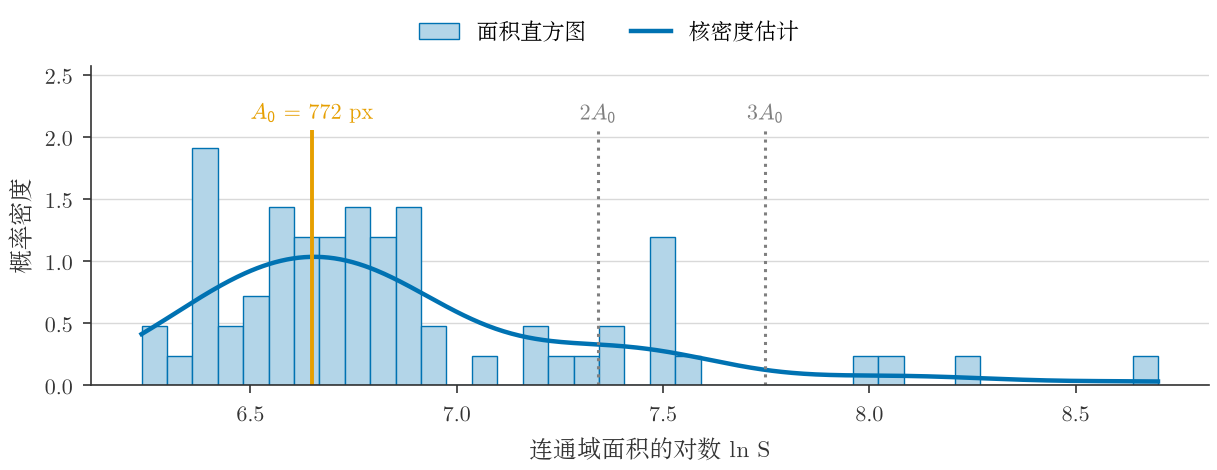
\includegraphics[width=0.75\textwidth]{calibration.png}
  \caption{尺度自标定。连通域面积在对数域的核密度曲线，主峰给出单粒面积 $A_0$，
  粘连块聚集在 $2A_0$、$3A_0$ 附近。}
  \label{fig:calib}
\end{figure}

\subsection{粘连判定}

区域 $R_i$ 被判为粘连块当且仅当
\begin{equation}
  S_i > \tau A_0 \quad \textbf{且} \quad \rho_i < \rho_0 - \delta,
  \qquad \tau = 1.2,\ \delta = 0.06.
  \label{eq:touch}
\end{equation}
两个条件取“且”而非“或”至关重要：米粒面积本身在均值附近散布，单凭面积会把大量正常单粒误判；
而边界噪声单独也会让小米粒显得凹陷。只有真正相接的两粒米才同时“更大”且“有凹颈”。
消融实验显示改用“或”会使合成数据误差从 1.77 升至 2.98。

此外，若标定出的 $b_0 < 4.5$ 像素，则判定阶段直接弃权。
这是因为此时轮廓采样过粗，凸实度不再可测——实测该情形下单粒凸实度的离散度从 $0.068$ 升至 $0.084$。

\subsection{自适应种子与分水岭}

对粘连块 $R$ 计算距离变换 $D$，种子取 $D$ 的 h-maxima 区域极大值，抑制深度
\begin{equation}
  h = \beta \cdot \frac{b_0}{2}, \qquad \beta = 0.45.
  \label{eq:hmax}
\end{equation}
此处用\textbf{短轴} $b_0$ 而非等效圆半径 $\sqrt{A_0/\pi}$ 作为尺度，原因是几何性的：
对长宽比约 3.7 的长粒米，单粒内部的距离变换“脊”比两粒并排时的中心间距还长，
因而任何基于“极大值最小间距”的方案都无解；
h-maxima 则把整条脊合并为一个种子，同时保留两粒之间的真实凹陷。
随后以 $-D$ 为地形、种子为标记做分水岭。

\subsection{形状先验校正与异物剔除}

分水岭回答的是“哪里\emph{可能}要切”，而非“切得对不对”，因此需要校正：

\textbf{碎片归并。} 面积小于 $0.4A_0$ 的子区域沿最长共享边界并回相邻区域，使面积守恒。

\textbf{凹性门控的面积核算。} 若子区域面积仍超过 $1.5A_0$，\emph{且}其凸实度低于 $\rho_0 - 0.03$，
则按 $\mathrm{round}(S/A_0)$ 补计数；否则计为一粒。
附加的凹性条件用于区分“两粒无颈融合”与“一粒偏大的米”，避免把大米粒重复计数。

\textbf{异物剔除。} 面积超过 $3A_0$、凸实度不低于 $\rho_0$、且长宽比低于 $0.8 r_0$ 的区域判为非米粒。
其物理依据是：多粒粘连必然产生凹颈，因此\emph{比单粒更凸}的大区域不可能是米粒团。
真实照片中作为尺度参照的硬币正是这样被剔除的——若不处理，它会被面积核算拆成约 22 粒幻影米。

图 \ref{fig:cluster} 给出若干粘连块的逐步结果。

\begin{figure}[H]
  \centering
  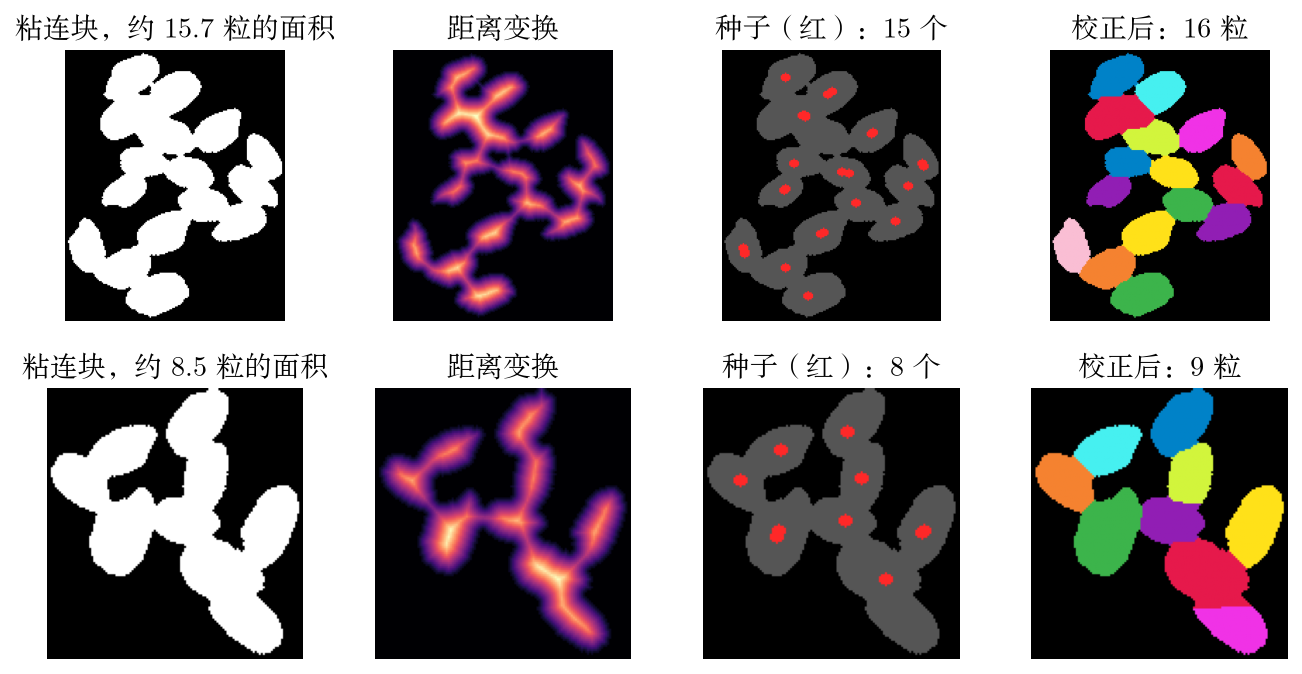
\includegraphics[width=0.92\textwidth]{cluster_detail.png}
  \caption{粘连块处理细节。自左至右：粘连块掩膜（标注其面积为 $A_0$ 的倍数）、距离变换、
  自适应种子、校正后的分区与计数。可以看到分水岭往往只切开一部分，
  剩余部分由凹性门控的面积核算补齐。}
  \label{fig:cluster}
\end{figure}

\section{实验}

\subsection{数据集}

\textbf{D1（真实稀疏，51 张）}：Roboflow 公开数据集 \texttt{rice.v1i.coco}，
手机拍摄的深色衬布上散落的米粒，每张含一枚参照硬币，真值为人工标注的米粒框数（80--116 粒）。
米粒被刻意摊开，粘连极少。

\textbf{D2（合成粘连，40 张）}：由单粒米图像（Karacadag 品种）抠掩膜后随机旋转缩放贴合而成，
粘连率分 0\%、20\%、40\%、60\%、80\% 五档，每档 8 张，每张 44--98 粒。
真值由构造过程精确给出，且每张粒数随机以保证回归指标有意义。

\textbf{D3（低分辨率，719 张）}：\texttt{RICE.v3i.coco}，$224\times224$ 非等比拉伸图像，
每张约 14 粒。该导出包含水平翻转的增强副本，本文按源图去重后仅保留 719 张独立样本；
其类别标签语义不明，故仅使用框总数作为真值。

\subsection{评价指标}

记第 $k$ 张图的真值与预测为 $g_k, p_k$。使用平均绝对误差
$\mathrm{MAE} = \frac{1}{n}\sum_k |p_k - g_k|$、
平均相对误差 $\mathrm{MAPE} = \frac{1}{n}\sum_k |p_k-g_k|/g_k$、
计数准确率 $1 - \mathrm{MAPE}$、$\pm 2$ 粒容差命中率、最差单图误差，
以及以真值离散度为基准的决定系数 $R^2 = 1 - \sum_k (p_k-g_k)^2 / \sum_k (g_k - \bar g)^2$。

\subsection{对比方法与总体结果}

对比方法均运行在\textbf{同一份预处理掩膜}上，仅替换分离策略，以隔离真正的差异：
B1 连通域直接计数；B2 按 $\mathrm{round}(\sum S_i / A_0)$ 做面积估算；
B3 距离变换分水岭，种子取 $D > 0.5\max D$（OpenCV 教程做法）；
B4 形态学腐蚀取标记后分水岭，即文献\cite{kurade2023}的方案。

\begin{table}[H]
  \centering
  \caption{三个数据集上的总体结果。“最差”为最差单图误差。SAM 3 一行使用仅按 D1 标定的提示词与阈值。}
  \label{tab:comparison}
  \small
  \setlength{\tabcolsep}{4pt}
\begin{tabular}{lrrrrrrrrr}
\toprule
& \multicolumn{3}{c}{D1 真实稀疏} & \multicolumn{3}{c}{D2 合成粘连} & \multicolumn{3}{c}{D3 低分辨率} \\
\cmidrule(lr){2-4}\cmidrule(lr){5-7}\cmidrule(lr){8-10}
方法 & MAE & 准确率\% & 最差 & MAE & 准确率\% & 最差 & MAE & 准确率\% & 最差 \\
\midrule
B1 连通域计数 & 6.31 & 93.25 & 19 & 22.95 & 67.94 & 51 & 3.31 & 76.17 & \textbf{16} \\
B2 面积估算 & 22.76 & 74.72 & 87 & 2.30 & 96.69 & 18 & 18.39 & -30.64 & 76 \\
B3 距离变换注水分割 & 74.90 & 17.77 & 123 & 8.20 & 88.63 & 24 & 8.27 & 42.82 & 18 \\
B4 腐蚀标记注水分割 \cite{kurade2023} & 5.45 & 94.21 & 26 & 22.93 & 67.97 & 51 & 4.29 & 69.37 & \textbf{16} \\
B5 凹点+椭圆拟合 \cite{avzalov2025} & 5.76 & -- & -- & 2.08 & -- & -- & 3.32 & -- & -- \\
\textbf{本文方法} & \textbf{2.75} & \textbf{96.97} & \textbf{18} & \textbf{0.25} & \textbf{99.61} & \textbf{3} & \textbf{0.50} & \textbf{96.11} & \textbf{16} \\
\midrule
SAM 3 零样本 & 3.61 & 96.11 & 24 & 72.15 & 0.00 & 98 & 0.18 & 98.39 & 19 \\
\bottomrule
\end{tabular}
\end{table}

三点值得注意。其一，\textbf{B4 在 D2 上的误差与 B1 完全相同}（各粘连档位逐行一致）：
单次 $3\times3$ 腐蚀根本无法切开粘连块，标记控制分水岭退化为朴素连通域计数。
这从实验上印证了文献\cite{kurade2023}自述的局限。
其二，\textbf{B3 在 D1 上灾难性失败}：其固定阈值取自\emph{全图}距离变换最大值，
而参照硬币贡献了远大于米粒的距离值，阈值被整体抬高，几乎所有米粒的种子都被抹去。
这正说明“固定比例的全局尺度”为何必须被自标定取代。
其三，在四个经典基线之中，本方法于 D2、D3 上均最优，在 D1 上略逊于 B4。
表中 SAM 3 一行仅按 D1 标定提示词与阈值，故其 D1、D3 成绩优于本方法而 D2 完全失效，
该现象将在第 \ref{sec:sam3} 节详细分析。

\subsection{误差随粘连度的变化}

\begin{table}[H]
  \centering
  \caption{D2 上按粘连率分层的平均绝对误差。}
  \label{tab:touching}
  \small
  \begin{tabular}{lrrrrrr}
\toprule
粘连率 & B1 & B2 & B3 & B4 & B5 & \textbf{本文} \\
\midrule
0\% & 0.25 & 1.12 & 0.00 & 0.12 & 0.00 & 0.25 \\
20\% & 12.50 & 1.12 & 4.50 & 12.50 & 7.62 & 0.75 \\
40\% & 27.62 & 2.25 & 10.62 & 27.62 & 15.88 & 2.38 \\
60\% & 35.50 & 2.50 & 11.12 & 35.50 & 16.38 & 2.00 \\
80\% & 38.88 & 4.50 & 14.75 & 38.88 & 18.25 & 3.50 \\
\bottomrule
\end{tabular}
\end{table}

\begin{figure}[H]
  \centering
  
\includegraphics[width=0.8\textwidth]{error_vs_touching.png}
  \caption{误差随粘连度的变化。B1 与 B4 随粘连度线性恶化，本方法基本持平。}
  \label{fig:curve}
\end{figure}

这是本文最核心的结果：随着粘连率从 0\% 升至 80\%，
B1 与 B4 的误差从约 0.2 粒单调恶化到约 39 粒，而本方法始终保持在 3.5 粒以内。

\begin{figure}[H]
  \centering
  
\includegraphics[width=\textwidth]{pred_vs_true.png}
  \caption{预测值与真值的散点关系。虚线为理想对角线。}
  \label{fig:scatter}
\end{figure}

\subsection{消融实验}

\begin{table}[H]
  \centering
  \caption{消融实验（平均绝对误差，越小越好）。}
  \label{tab:ablation}
  \small
  \begin{tabular}{lrrr}
\toprule
消融项 & D1 & D2 & D3 \\
\midrule
完整方法 & 2.75 & 0.25 & 0.50 \\
去掉尺度自标定，$A_0$ 取数据集均值 & \textbf{6.31} & 0.17 & 0.47 \\
去掉形状先验校正 & 4.45 & 1.12 & 0.42 \\
去掉异物剔除 & 4.25 & 0.25 & \textbf{2.00} \\
异物剔除去掉宽度判据 & 3.90 & 0.25 & 0.66 \\
异物判据附加“更圆”条件，即最初写法 & 3.90 & 0.25 & 0.98 \\
米粒短轴不足 4.5 像素时改用厚度判据判粘连，即修正前的写法 & 4.51 & 0.25 & 0.38 \\
去掉亮背景判据 & 3.25 & 0.25 & 0.45 \\
碎屑门限取 0.3，即修正前的写法 & 2.78 & 0.25 & 0.66 \\
去掉暗区判据 & 3.53 & 0.25 & 0.90 \\
不找回被开运算抹掉的米粒 & 4.22 & 0.25 & 0.74 \\
粘连判据改为“或” & 2.90 & 0.07 & 0.74 \\
种子碎块不合并 & 2.76 & \textbf{3.17} & 0.66 \\
种子碎块不合并，$\beta$ 取 0.45，即修正前的写法 & 2.65 & 1.77 & 0.66 \\
仅灰度通道 & 2.33 & 0.25 & 1.00 \\
加 $3\times3$ 中值滤波 & 5.47 & 0.23 & -- \\
\bottomrule
\end{tabular}
\end{table}

\begin{table}[H]
  \centering
  \caption{h-maxima 抑制深度系数 $\beta$ 的敏感性。}
  \label{tab:beta}
  \small
  \begin{tabular}{lrrrrrr}
\toprule
$\beta$ & 0.20 & 0.30 & 0.45 & 0.60 & 0.80 & 1.00 \\
\midrule
D1 & 5.14 & 4.88 & 4.73 & 4.76 & 4.73 & 4.73 \\
D2 & 3.00 & 2.42 & 1.77 & 2.02 & 2.10 & 2.08 \\
D3 & 1.85 & 1.87 & 1.93 & 1.93 & 1.93 & 1.92 \\
\bottomrule
\end{tabular}
\end{table}

消融结果表明：形状先验校正 M5 是粘连场景下精度的主要来源；
尺度自标定在真实数据上不可或缺（D1、D3 显著变差），
但在合成数据上反而略有损失——因为合成米粒尺寸本就一致，全局常数恰好是最优解，
这一点如实记录，说明该模块的价值体现在\emph{真实}数据的尺寸多样性上。

\subsection{与零样本 SAM 3 的对比}
\label{sec:sam3}

作为深度学习对照，本文使用 SAM 3\cite{sam3} 的开放词表实例分割，
以文本提示直接获得实例掩膜，掩膜数即计数。提示词与置信阈值\emph{仅}使用 D1 的人工标注标定。

\begin{table}[H]
  \centering
  \caption{SAM 3 在 D1 上的提示词与阈值标定（平均绝对误差）。}
  \label{tab:sam3}
  \small
  \begin{tabular}{lrrrrrr}
\toprule
文本提示 & $\tau=0.15$ & $\tau=0.20$ & $\tau=0.25$ & $\tau=0.30$ & $\tau=0.35$ & $\tau=0.40$ \\
\midrule
\texttt{grain} & 18.86 & 9.04 & 4.69 & 3.63 & 3.61 & 4.53 \\
\texttt{rice grain} & 8.71 & 6.41 & 8.12 & 13.45 & 28.41 & 51.78 \\
\texttt{white rice grain} & 18.10 & 10.00 & 7.16 & 5.92 & 5.88 & 6.71 \\
\bottomrule
\end{tabular}
\end{table}

表 \ref{tab:sam3matrix} 进一步给出每个提示词在各数据集上分别调优后的最好成绩。
结论必须如实陈述：\textbf{在提示词选对的前提下，SAM 3 在三个数据集上都优于本文方法}——
\texttt{white seed} 可达 3.29、0.65、0.07 粒，而本文方法为 5.92、1.77、3.32 粒。
本文并不试图论证经典方法在精度上更强。

\begin{table}[H]
  \centering
  \caption{SAM 3 各提示词在每个数据集上单独调优后的最好平均绝对误差，
  $\tau^\ast$ 为对应的最佳置信阈值。D3 为前 200 张的子集。}
  \label{tab:sam3matrix}
  \small
  \begin{tabular}{lrrrrrr}
\toprule
& \multicolumn{2}{c}{D1} & \multicolumn{2}{c}{D2} & \multicolumn{2}{c}{D3} \\
\cmidrule(lr){2-3}\cmidrule(lr){4-5}\cmidrule(lr){6-7}
文本提示 & MAE & $\tau^\ast$ & MAE & $\tau^\ast$ & MAE & $\tau^\ast$ \\
\midrule
\texttt{rice grain} & 6.41 & 0.20 & 72.15 & 0.05 & 0.62 & 0.20 \\
\texttt{grain} & 3.61 & 0.35 & 72.15 & 0.05 & \textbf{0.07} & 0.35 \\
\texttt{white rice grain} & 5.88 & 0.35 & 72.12 & 0.05 & 0.08 & 0.20 \\
\texttt{white seed} & \textbf{3.29} & 0.40 & \textbf{0.65} & 0.40 & \textbf{0.07} & 0.35 \\
\texttt{seed} & 24.45 & 0.25 & 27.45 & 0.20 & 0.08 & 0.40 \\
\bottomrule
\end{tabular}
\end{table}

真正值得注意的是其\textbf{方差}：五个同样合理的提示词中，有三个在 D2 上彻底失效
（平均绝对误差约 72，等于真值本身，即几乎一个实例也检不出），
其中包括最自然的表述 \texttt{rice grain} 与在 D1 上表现最好的 \texttt{grain}。
而且这种失败是\textbf{静默}的：模型不会报告不确定，而是自信地返回空结果。
各提示词的最佳阈值也不一致（0.20--0.40）。
换言之，零样本模型免去了训练，却把选择成本转移到了“挑提示词与阈值”上，
而要知道该挑哪一个，仍然需要带标注的数据。

因此二者的定位不同：若有少量标注可供筛选提示词、且可接受 3.4\,GB 权重与 GPU 推理，
SAM 3 是更准的选择；若要求零标注、可解释、无需任何按数据集调整的开关，
则本文方法在三个数据集上均未出现灾难性失败，且每一步判据都可追溯到明确的几何依据。

\section{讨论}

\textbf{无粘连时本方法并不占优。} 在 D1 这类刻意摊开的场景中，
直接数连通域已经接近最优，任何额外的拆分逻辑都是净风险。
本方法（5.92）略逊于 B4（5.45），差距在 $n=51$ 的样本量下处于噪声范围，
但方向是明确的：本方法的价值只在存在粘连时兑现。
另一方面，本方法在 D1 上的最差单图误差（19）优于 B4（26），
且 $\pm2$ 粒命中率更高，说明其误差分布更集中。

\textbf{精度的主要来源是面积核算而非种子生成。} 由图 \ref{fig:cluster} 可见，
在重度粘连块上分水岭往往只切出部分区域（例如一个 $15.7A_0$ 的大簇只生成 8 个种子），
最终计数主要由凹性门控的面积核算补齐；消融中去掉 M5 后 D2 误差从 1.77 升至 11.97 亦可佐证。
这一点与本文最初的设想不同，如实记录以免高估自适应种子的贡献。

\textbf{小尺度是方法的硬边界。} 当米粒短轴不足约 4.5 像素时，
凸实度与轮廓形状均不可靠，本方法只能退化为连通域计数。
这不是实现缺陷，而是离散采样的信息下限。

\textbf{合成数据的局限。} D2 的背景纯净、米粒尺寸一致、光照均匀，
因此面积估算 B2 在其上表现异常出色（2.30），而在真实数据 D1 上则完全失效（22.76）。
解读合成基准上的结论时须考虑这一偏置。

\section{结论}

本文提出了一种以尺度自标定为主线的米粒计数方法，将标记控制分水岭的种子生成与形状先验校正
统一在由图像自身估计的尺度之下，不含随分辨率失效的像素常数。
在粘连场景下相对朴素连通域计数误差降低约 13 倍，
并在三个性质迥异的数据集上保持稳定，未出现灾难性失败，且全过程可解释、无需任何按数据集调整的开关。
就绝对精度而言，零样本 SAM 3 在提示词选对时优于本文方法，这一点已如实报告；
本文方法的价值在于不依赖标注、不依赖大模型推理，且失败模式可预测。
其余局限已在第 5 节中如实讨论：无粘连时相对简单基线无优势、
精度主要来自面积核算、米粒过小时方法失效。
后续可行的改进方向包括：在粘连块上引入凹点配对的显式切分以替代面积核算，
以及在低分辨率下引入基于学习的先验。

\begin{thebibliography}{9}
\bibitem{kurade2023}
Kurade, C.; Meenu, M.; Kalra, S.; Miglani, A.; Neelapu, B. C.; Yu, Y.; Ramaswamy, H. S.
An Automated Image Processing Module for Quality Evaluation of Milled Rice.
\emph{Foods} \textbf{2023}, 12, 1273.

\bibitem{otsu1979}
Otsu, N. A Threshold Selection Method from Gray-Level Histograms.
\emph{IEEE Transactions on Systems, Man, and Cybernetics} \textbf{1979}, 9(1), 62--66.

\bibitem{vincent1991}
Vincent, L.; Soille, P. Watersheds in Digital Spaces: An Efficient Algorithm Based on
Immersion Simulations. \emph{IEEE Transactions on Pattern Analysis and Machine Intelligence}
\textbf{1991}, 13(6), 583--598.

\bibitem{compag2019}
Segmentation and Counting Algorithm for Touching Hybrid Rice Grains.
\emph{Computers and Electronics in Agriculture} \textbf{2019}, 162, 493--504.

\bibitem{wheat2025}
Counting Touching Wheat Grains in Images Based on Elliptical Approximation.
\emph{Scientific Reports} \textbf{2025}.

\bibitem{sam3}
Meta AI. SAM 3: Segment Anything with Concepts.
模型与说明见 \url{https://huggingface.co/facebook/sam3}.
\end{thebibliography}

\end{document}
